\chapter{Determined protein structures}
This section describes all test-targets which I have attempted to fold using the methodologies presented in the previous chapters.

\section{Barley Chymotrypsin Inhibitor II}

An especially interesting target in this study is the barley chymotrypsin inhibitor II (CI-2). CI-2 is a 63 residue protein which consists of an $\alpha$-helix which connects via a very flexible handle to a small $\beta$-sheet region.

The chemical shifts data was obtained using a fully automated procedure.
The ADAPT-NMR [REF XX] protocol was used to record all necessary NMR data and automatically assign the chemical shifts.
Data collection and assignment was completed in only 11 hours with minimal human intervention.
As we demonstrate, a structure could be determined computationally from these chemical shifts in only two days running on 12 cores.



\subsection{Computational methodology}
Several folding protocols were tried for this protein. All runs were performed as 72 independent trajectories which ran for 50 mio MC steps (iterations). Sampling was carried out using either TorusDBN or TorusDBN-CS to bias the backbone moves and the PROFASI force field was used in all simulations. Three simulations used an energy function based on CamShift using a cauchy distribution with variable $\gamma$ value as energy function. Additionally, three simulations used a potential on the radius of gyration to restrict the sampling to only compact structures. MUNINN was was set to multicanonical sampling and the thermodynamic beta-range was set to between 0.6 and 1.1, corresponding to a temperature range of 272K to 500K. The MC moves were set to 49\% CRISP moves, 2\% pivot moves and 49\% uniform side chain moves.


\begin{table}[h]
    \caption{Protocols used in the folding of the CI-2 protein and success rates.}
    \begin{center}
    \begin{threeparttable}
    \begin{tabular}{l l l l l l}
        Sampling        & Force Field   & CS Energy         & Correct fold\tnote{a} & Iterations/day\tnote{b}\\\hline
          TORUS-CS + PP\tnote{c} & PROFASI       & CamShift          & 13            & $10 \times 10^6$ \\
          TORUS-CS      & PROFASI       & CamShift          & 15            & $11 \times 10^6$\\
          TORUS         & PROFASI       & CamShift          & 0             & $11 \times 10^6$\\
 TORUS-CS + PP\tnote{c} & PROFASI       & None              & 4\tnote{d}      & $49 \times 10^6$\\
 TORUS-CS\tnote{e}+ PP\tnote{c} & PROFASI      & None              & 0             & $49 \times 10^6$\\
          TORUS-CS      & PROFASI       & None              & 0             & $49 \times 10^6$\\
          TORUS         & PROFASI       & None              & 0             & $49 \times 10^6$\\
    \end{tabular}
    \begin{tablenotes}
        \item[a] Number of threads with a CA-RMSD of $<5$ \AA\ (using all residues).\\
        \item[b] Numbers are \textit{per} thread.
        \item[c] PP denote the use of a radius of gyration potential.\\
        \item[d] Structures with the lowest energy did not correspond to the native structure in this run.\\
        \item[e] This run was carried out using TorusDBN-CS trained using only high-quality X-ray structures.
    \end{tablenotes}
    \end{threeparttable}
    \end{center}
    \label{tab:ci2}
\end{table}
\subsection{Folding results}
Three of the 7 attempted simulation types sample structures close to the experimental X-ray structure 1YPA (here loosely defined as a CA-RMSD $<5$ \AA\ for all CA atoms. Results are summarized n thable
None of the simulations that sample from TorusDBN (not chemical shift biased) are able to sample the correct fold.

Furthermore, it was noted, that simulations that sample from either TorusDBN or TorusDBN-CS with only the PROFASI force field as energy function do not generate compact structures.
To overcome this deficiency, additional simulations were carried out using a radius of gyration potential.
In the case of sampling from TorusDBN-CS, the radius of gyration potential is enough to get a few samples with the correct fold. Here four of 72 threads would generate the correct fold, but unfortunately the lowest energy structures were found around 8-11 \AA\ CA-RMSD. Evidently, the PROFASI force field alone is not accurate enough to describe the native CI-2 structure.
Three simulations were performed with an energy term based on CamShift in addition the PROFASI force field.
Demonstrably, the increased accuracy from a better energy function cause increased sampling around the native state.

Due to a very flexible region of CI-2 (residues 33 to 42), and somewhat flexible tails the residue range used to calculate CA-RMSD values is restricted to residue 4-34,43-63 in the following.
All runs were carried out on 3 24-core AMD Opteron 6172 servers running at 2.1 GHz. 

A run similar to the most successful was also run carried out on a faster a 12-core Intel X5675 node running at 3.07 GHz (using new random seeds).
This simulation took two days, with a total of 2 out of 12 threads successfully identifying the native structure as having the lowest energy.
This simulation yielded a lowest energy structure a 2.76 \AA~CA-RMSD from the X-ray structure, and a lowest RMSD structure at 1.11 \AA.

The lowest RMSD was further refined by Lars Bratholm to a CA-RMSD of only 1.1 which took 24 hours on 8 cores.


\begin{figure}%
    \centering
    \subfloat[NMR structure (red)]{
        {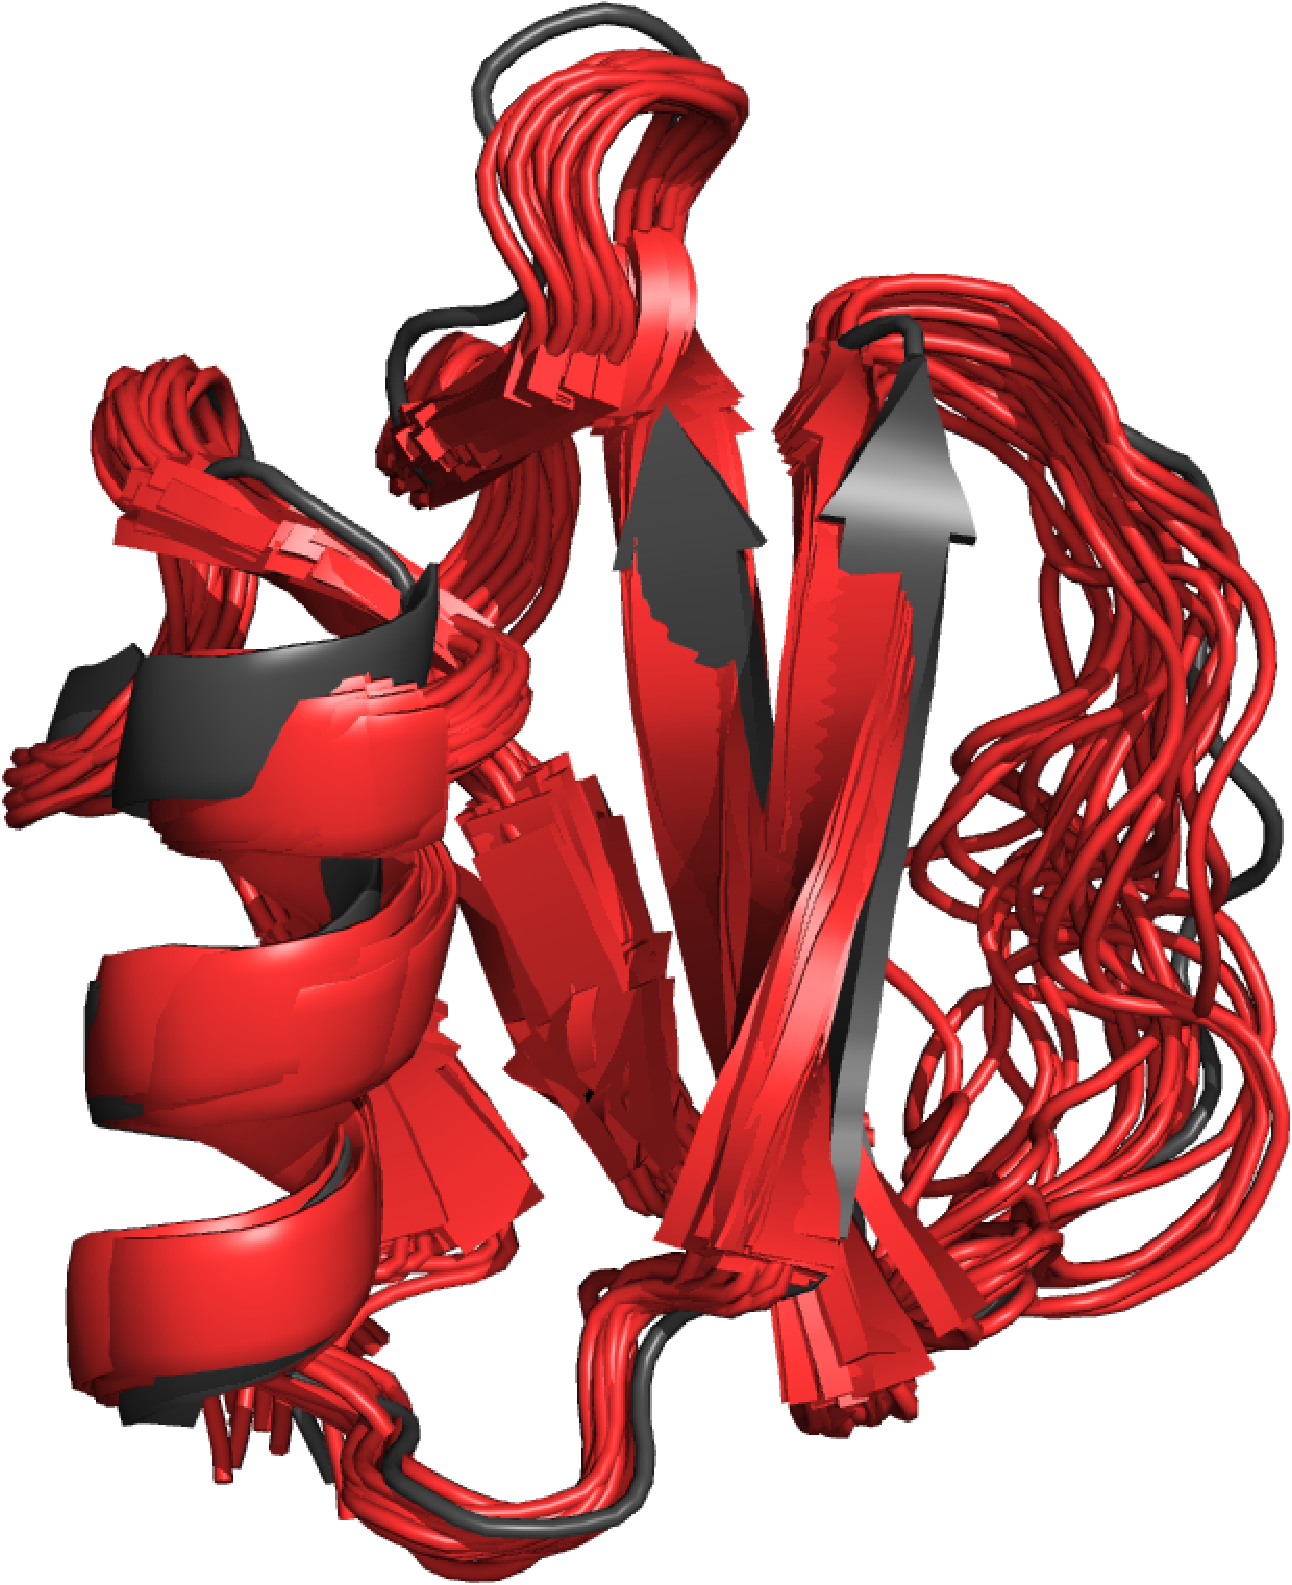
\includegraphics[width=0.3\textwidth]{figures/ci2_pymol/crystal_nmr_trim.pdf}}
    }
    \subfloat[Lowest RMSD structure (blue)]{
        {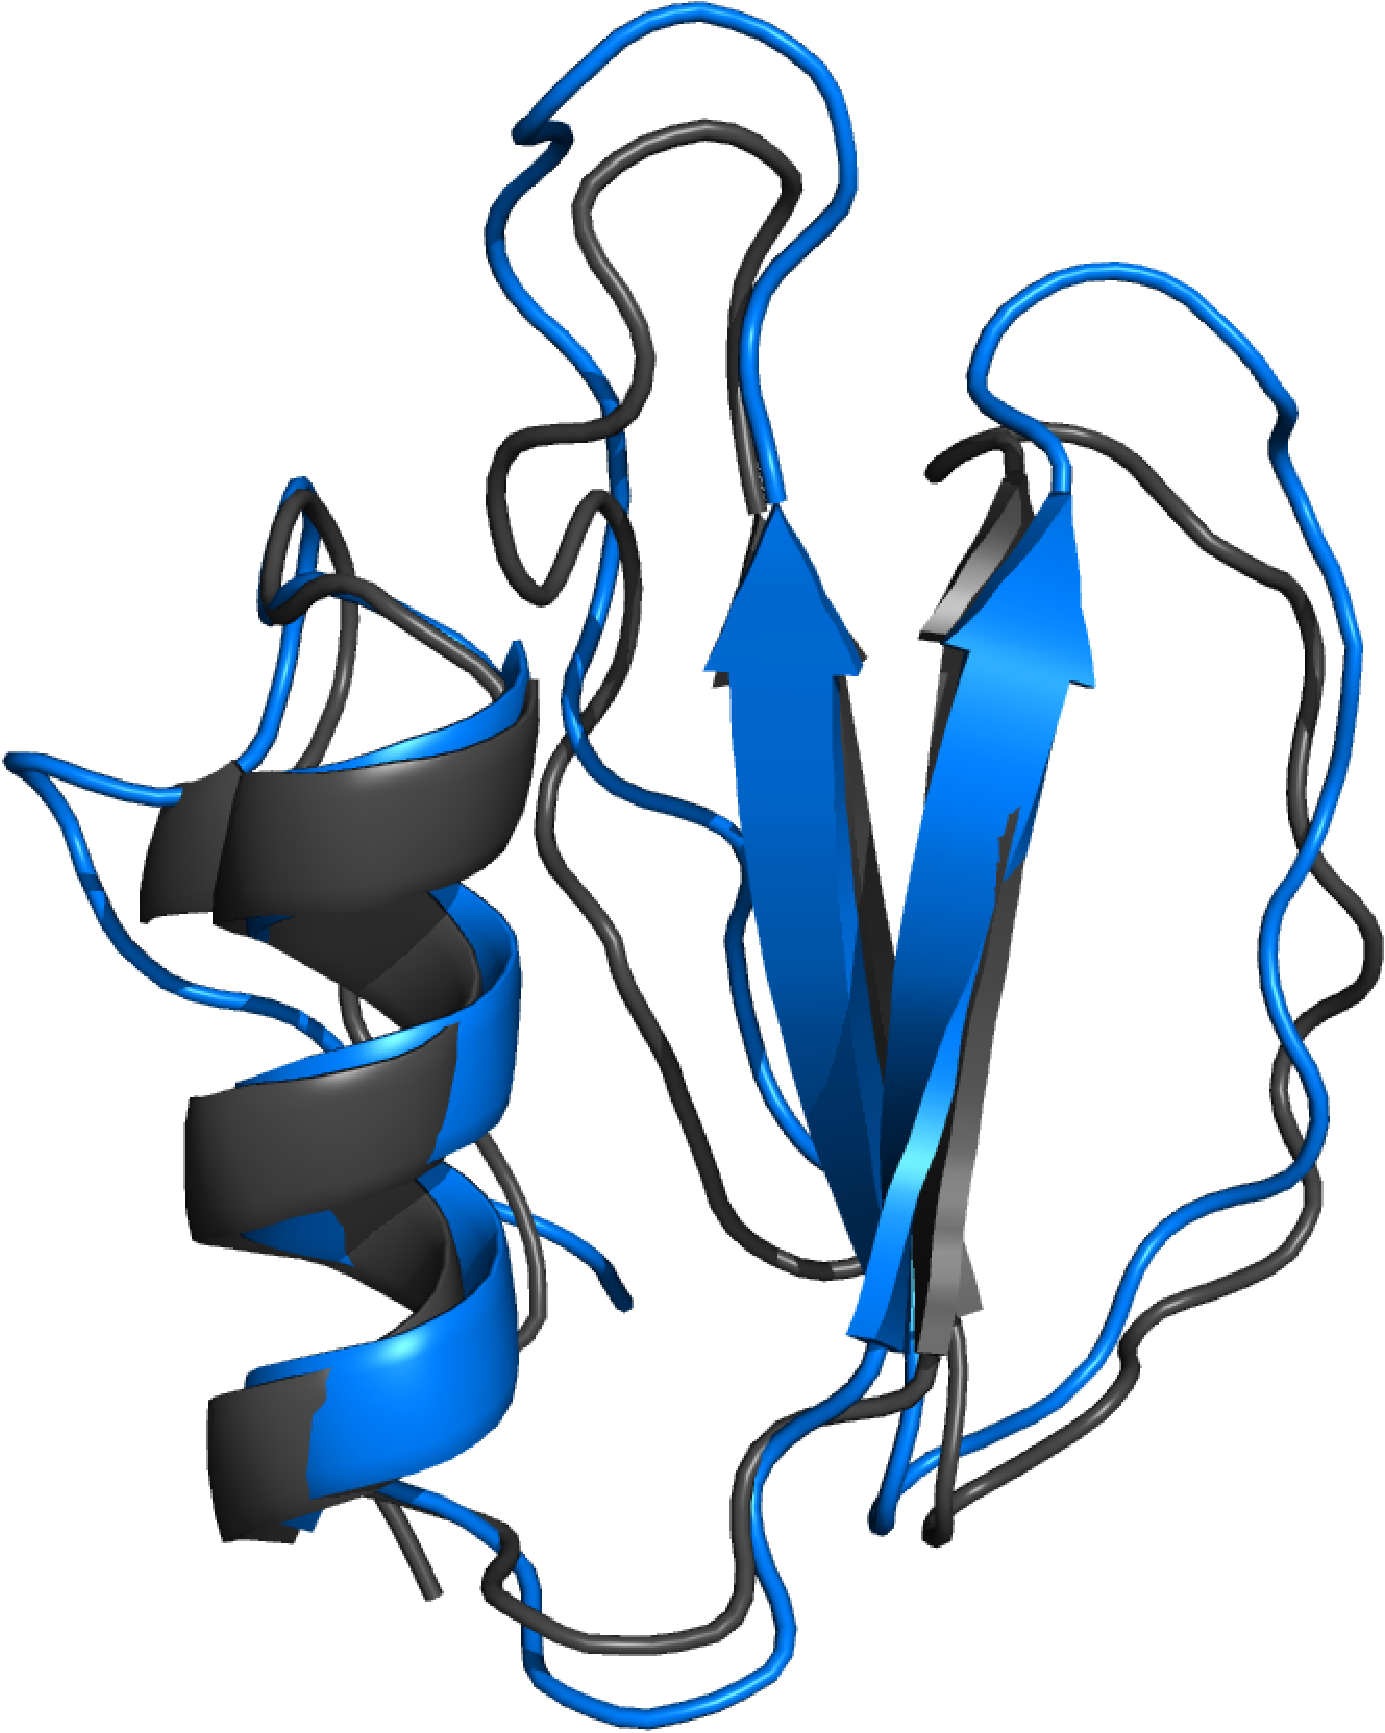
\includegraphics[width=0.3\textwidth]{figures/ci2_pymol/crystal_lowest_rmsd_trim.pdf}}
    }
    \subfloat[Lowest energy structure (green)]{
        {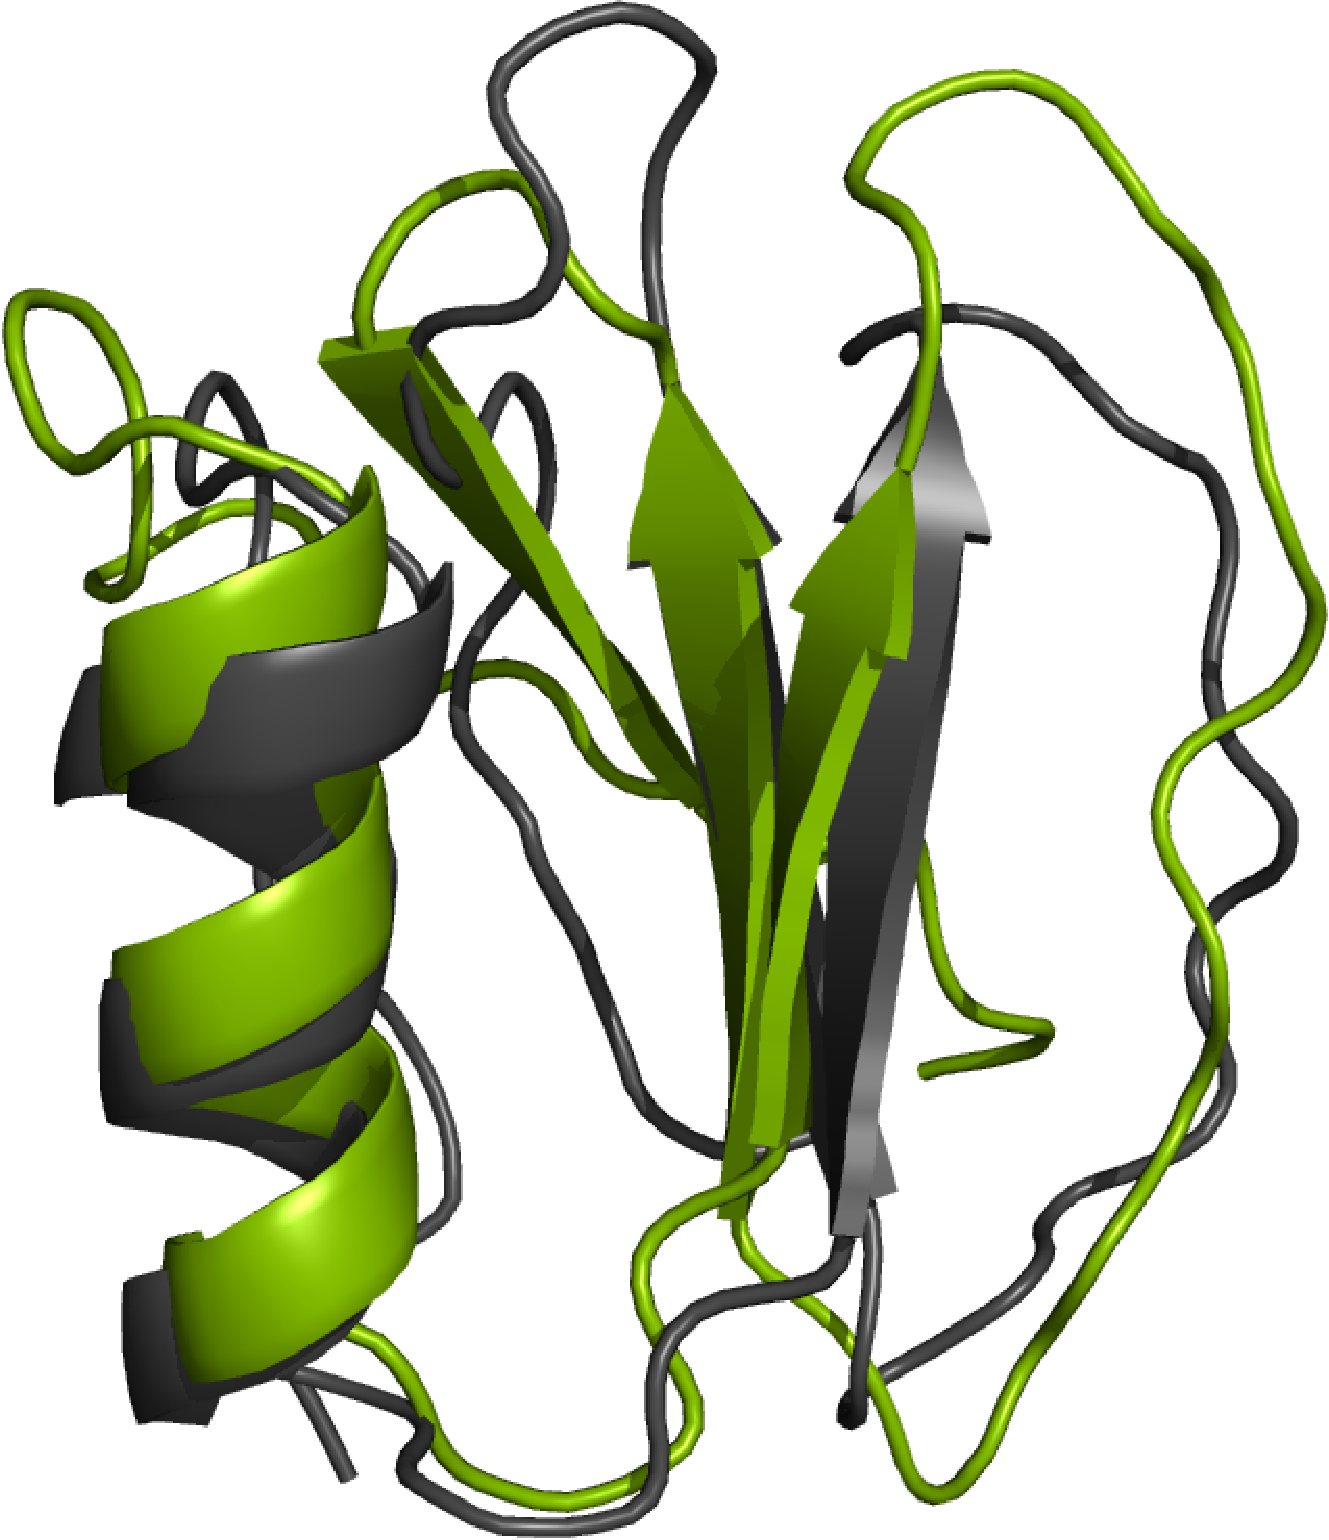
\includegraphics[width=0.3\textwidth]{figures/ci2_pymol/crystal_lowest_energy_trim.pdf}}
    }
    \caption{Structures compared to the X-ray structure 1YPA. All structures are aligned using the residues 12-32,43-52. (a) shows the 3CI2 structure NNR structure. Note the flexible domain which is excluded from the fit-range. (b) Shows the lowest RMSD structure (1.113 \AA RMSD). (c) shows the lowest energy sample (2.76 \AA RMSD). }
    \label{fig:ci2}%
\end{figure}







\section{Folding of small proteins (\textless 100 AA)}


\begin{table}[h]
    \caption{Folded structure.}
    \begin{center}
    \begin{threeparttable}
    \begin{tabular}{l l l l l  l l}
Name                & Lengh    & Type & PDB     & RefDB     & RMSD-range    & Final RMSD  \\\hline
Protein G           & 56       & a/b & 2OED    & 2575      & All           & 1.0           \\
% Can't find data for SMN Tudor Domain :( :( :( :( :(, only the 3.3 number :(
% SMN Tudor Domain    & 59       & a/b & 1MHN    & 4899      & 5-54          & 3.3       \\
Engrailed Homeodomain & 61     & B   & 1ENH    & 15536     & 8-53          & 1.1           \\
CI-2                & 63       & a/b & 1YPA    & N/A\tnote{a}& 4-34,43-63  & 2.6          \\
FF Domain           & 71       & a/b & 1UZC    & 5537      & 11-67         & 10.2*          \\
Ubiquitin           & 76       & a/b & 1UBI    & 17769     & 1-70          & 3.8
    \end{tabular}
    \begin{tablenotes}
    \item[a] Using automatically assigned data obtained from Kaare Theilum (personal communitcation - see \url{https://github.com/andersx/cs-proteins}).
    \end{tablenotes}
    \end{threeparttable}
    \end{center}
    \label{tab:folding_small}
\end{table}

\section{Folding of larger proteins (\textgreater 100 AA)}

This section presents folding results on a set of larger proteins (\textgreater 100 AA) with known structures. It is worth to note, that using sparse NMR data, only three structures \textgreater 200 residues have been determined: Alg13 (201 AA), Rhodopsin (225 AA) and MBP (376 AA) using the Rosetta program with the "resolution-adapted structural recombination" (RASREC) protocol

Alg13 was solved using backbone chemical shifts only 52 NOE, to an CA-RMSD of 4 \AA~to the experimental NMR structure (2jzc).
Rhodopsin was folded to an CA-RMSD of 1.6 \AA~to the X-ray structure using 215 NOE restraints, backbone chemical shifts chemical shifts and RDCs.
The MBP protein is a two-domain protein of 376 residues.
MBP was folded to an RMSD of 3.6 \AA~using 1235 NOE restraints, backbone chemical shifts chemical shifts and RDCs.
The NOEs corresponded to 55\% yield of restraints, which, however mostly were not automatically assigned.
An attempt to use only automatically assigned NOEs yielded 455 restraints, which corresponds to a yield of 20\%. Using these, however, the MBP structure could only be determined to a total CA-RMSD of 12.3 \AA.
The N-terminal domain was converged to 2.7 \AA, but the C-terminal domain and the angle between the two domains was incorrectly folded.

\subsection{Folding protocol}
The folding protocols used in the following was a two stage simulation. First folding, then refinement.



\subsubsection{Initial folding stage:}
\begin{lstlisting}
./phaistos --aa-file rhodopsin.aa \
  --iterations 50000000 \
  --threads 72 \
  --monte-carlo-muninn 1 \
  --monte-carlo-muninn-min-beta 0.6 \
  --monte-carlo-muninn-max-beta 1.1 \
  --monte-carlo-muninn-independent-threads 1 \
  --monte-carlo-muninn-weight-scheme multicanonical \
  --backbone-dbn-torus-cs 1 \
  --backbone-dbn-torus-cs-initial-nmr-star-filename \
                                      rhodopsin.str \
  --energy-profasi-cached 1 \
  --energy-isd-dist 1 \
  --energy-isd-dist-likelihood square_well \
  --energy-isd-dist-data-filename noe_ilv.txt \
  --energy-isd-dist-sample-gamme 0 \
  --energy-isd-dist-sample-sigma 0 \
  --energy-isd-dist-weight 0.0078125 \
  --move-backbone-dbn 1 \
  --move-backbone-dbn-weight 0.08 \
  --move-backbone-dbn-implicit-energy 1 \
  --move-crisp-dbn-eh 1 \
  --move-crisp-dbn-eh-weight 0.42 \
  --move-sidechain-uniform 1 \
  --move-sidechain-uniform-weight 0.5
\end{lstlisting}

\subsubsection{Refinement protocol:}

The 

\begin{lstlisting}
./phaistos --pdb-file rhodopsin_lowest_energy1.pdb \
  --init-from-pdb 1 \
  --iterations 2000000 \
  --threads 8 \
  --monte-carlo-metropolis-hastings 1 \
  --monte-carlo-metropolis-hastings-declash-on-reinitialize 0 \
  --backbone-dbn-torus-cs 1 \
  --backbone-dbn-torus-cs-initial-nmr-star-filename \
                                      rhodopsin.str \
  --energy-profasi-cached 1 \
  --energy-pp-compactness 1 \
  --move-backbone-dbn 1 \
  --move-backbone-dbn-weight 0.08 \
  --move-backbone-dbn-implicit-energy 1 \
  --move-crisp-dbn-eh 1 \
  --move-crisp-dbn-eh-weight 0.42 \
  --move-sidechain-uniform 1 \
  --move-sidechain-uniform-weight 0.5
\end{lstlisting}


\subsection{Rhodopsin (225 residues)}

\begin{figure}%
    \centering
    \subfloat[Energy-scoring during folding stage.]{
        {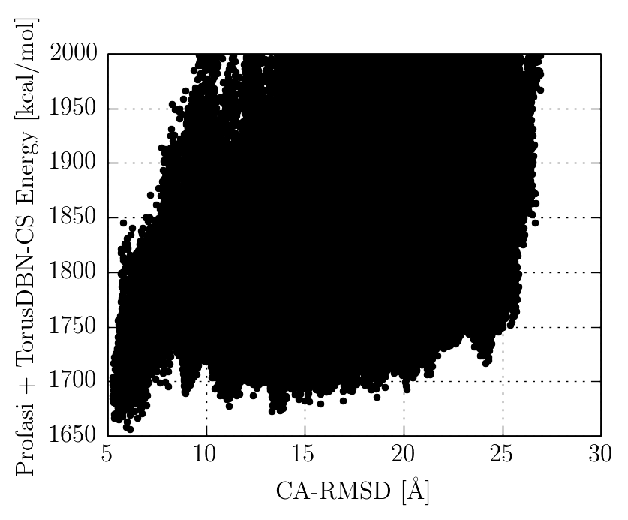
\includegraphics[width=0.4\textwidth]{figures/rhodopsin_figures/folding_data.pdf}}
    }\quad
    \subfloat[Energy-scoring during refinement stage.]{
        {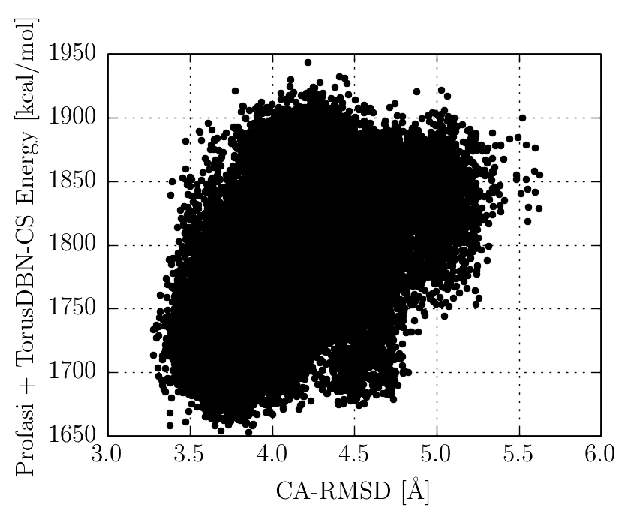
\includegraphics[width=0.4\textwidth]{figures/rhodopsin_figures/refinement_data.pdf}}
    }\\
%    \subfloat[Bottom view of folding stage lowest energy sample (blue).]{
%        {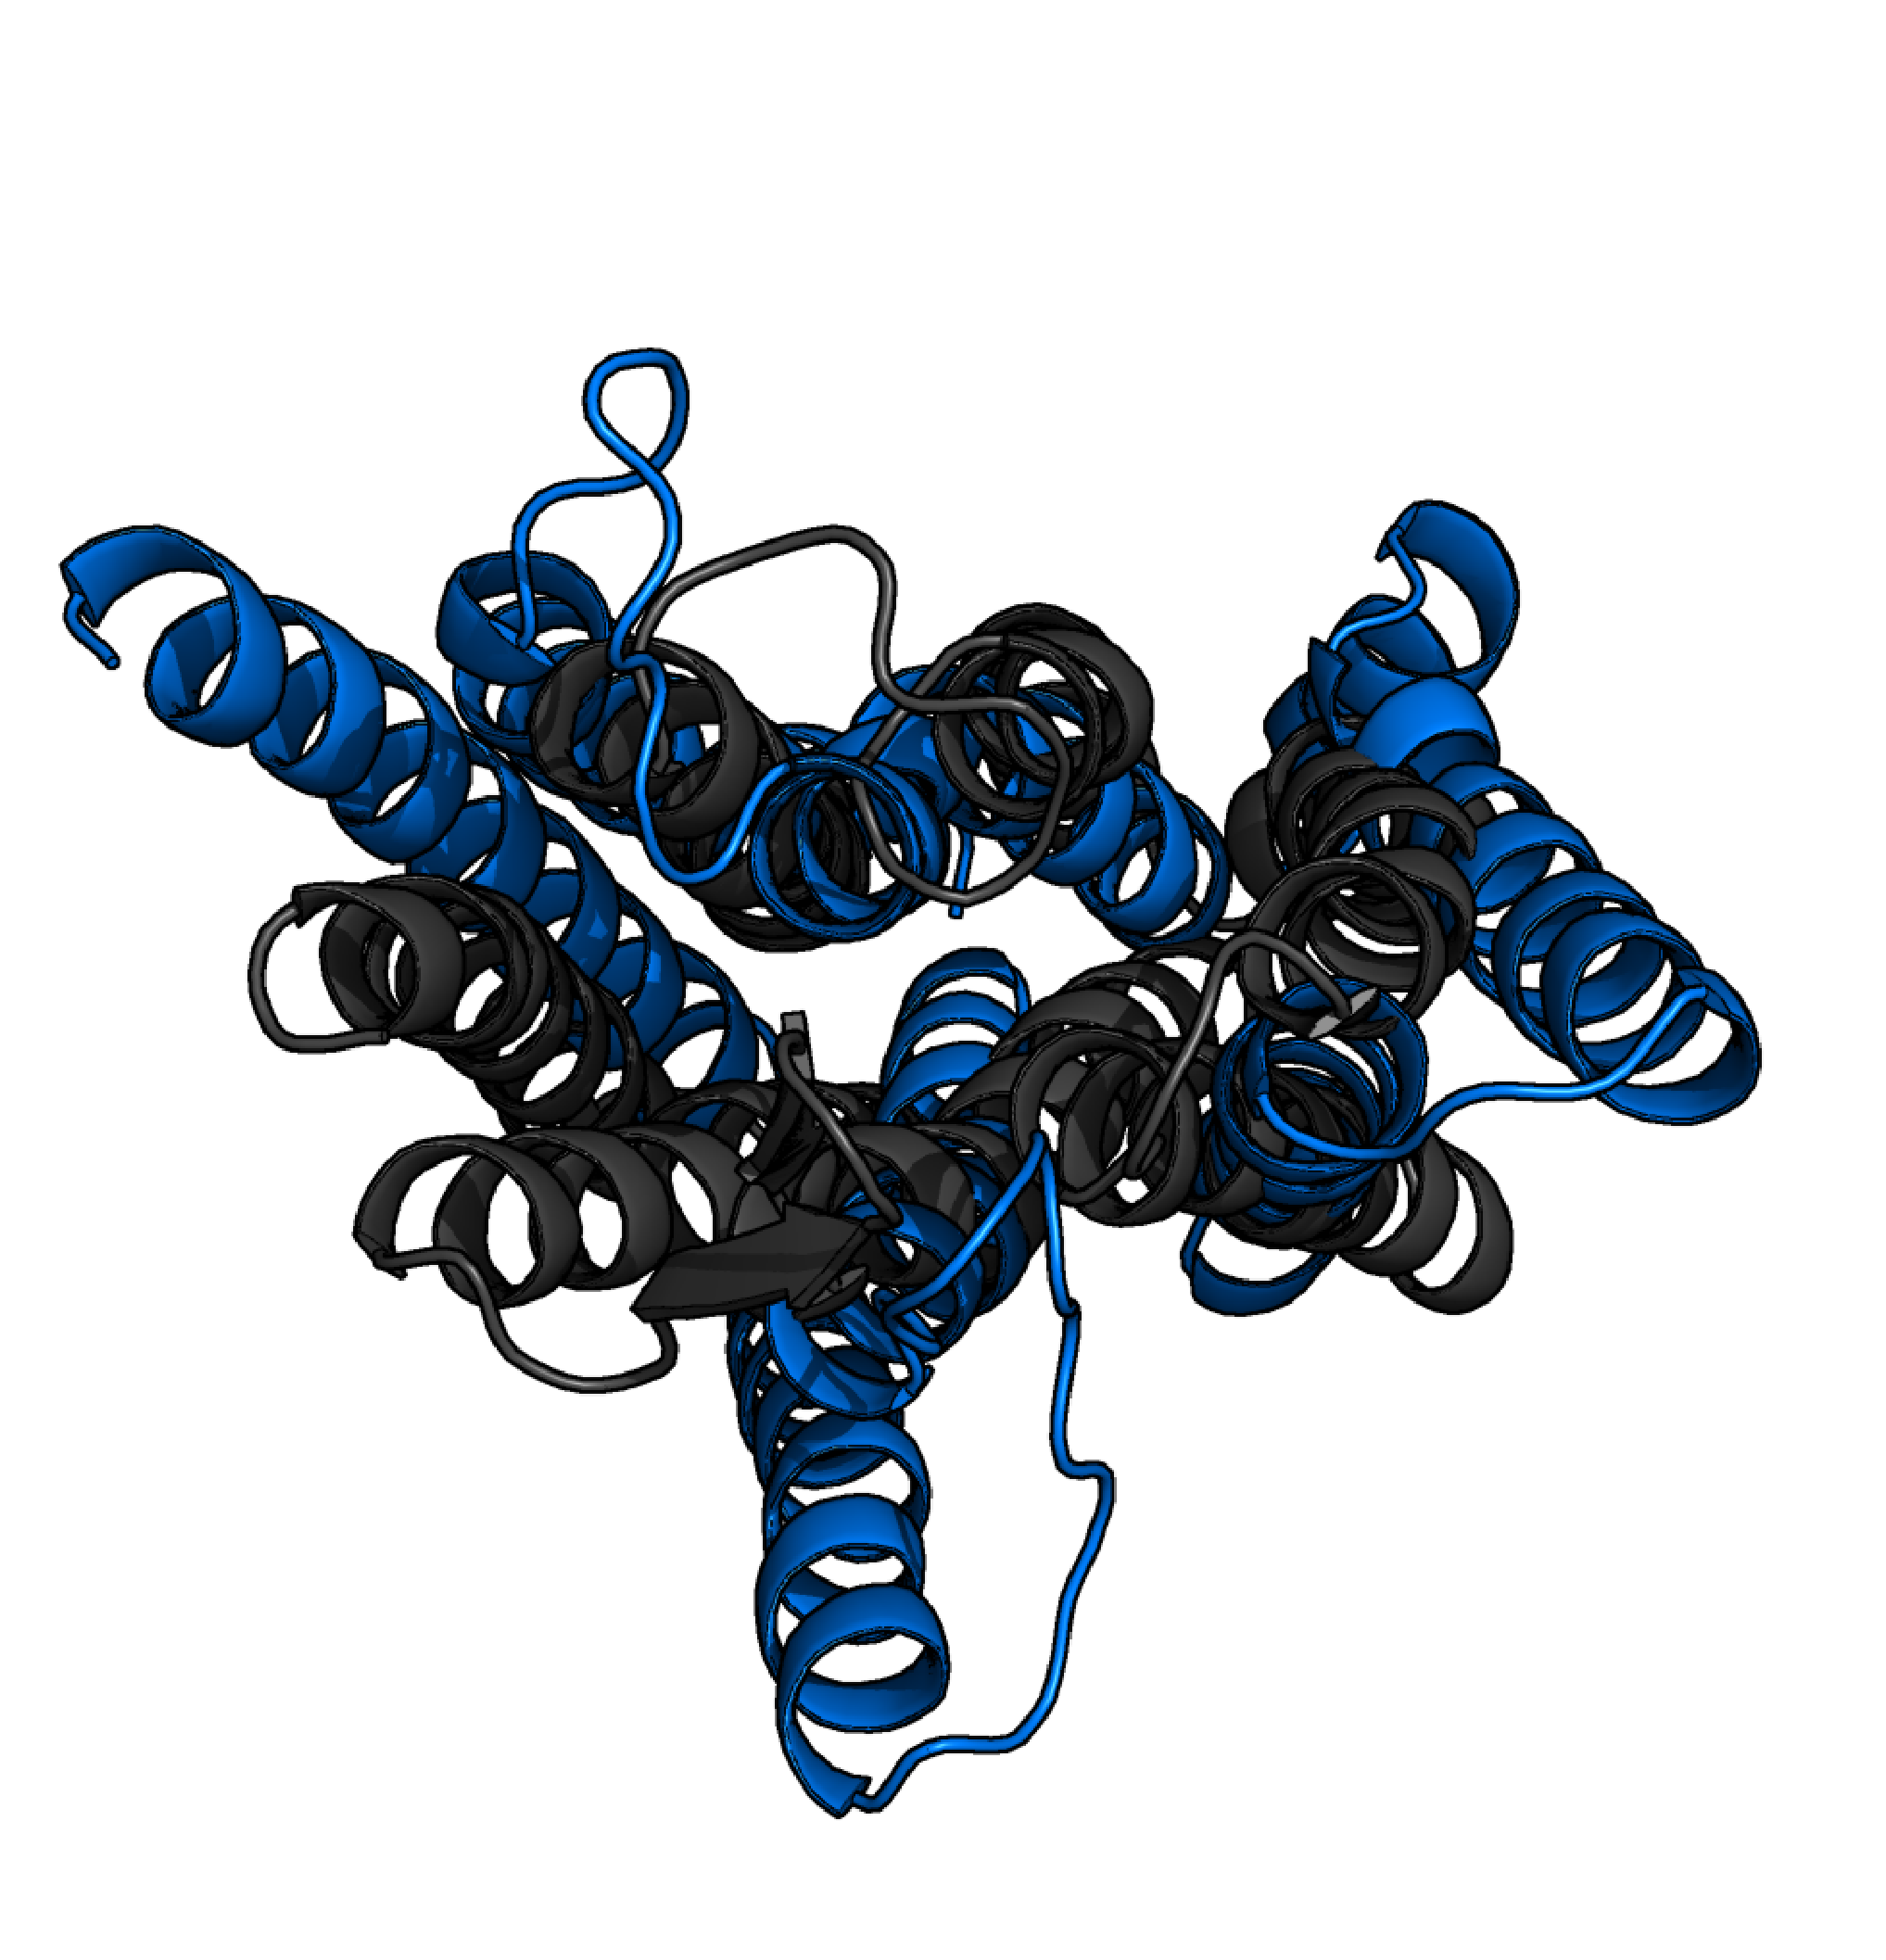
\includegraphics[width=0.4\textwidth]{figures/rhodopsin_figures/folding_bottom.pdf}}
%    }\quad
%    \subfloat[Bottom view of refinement stage lowest energy sample (red).]{
%        {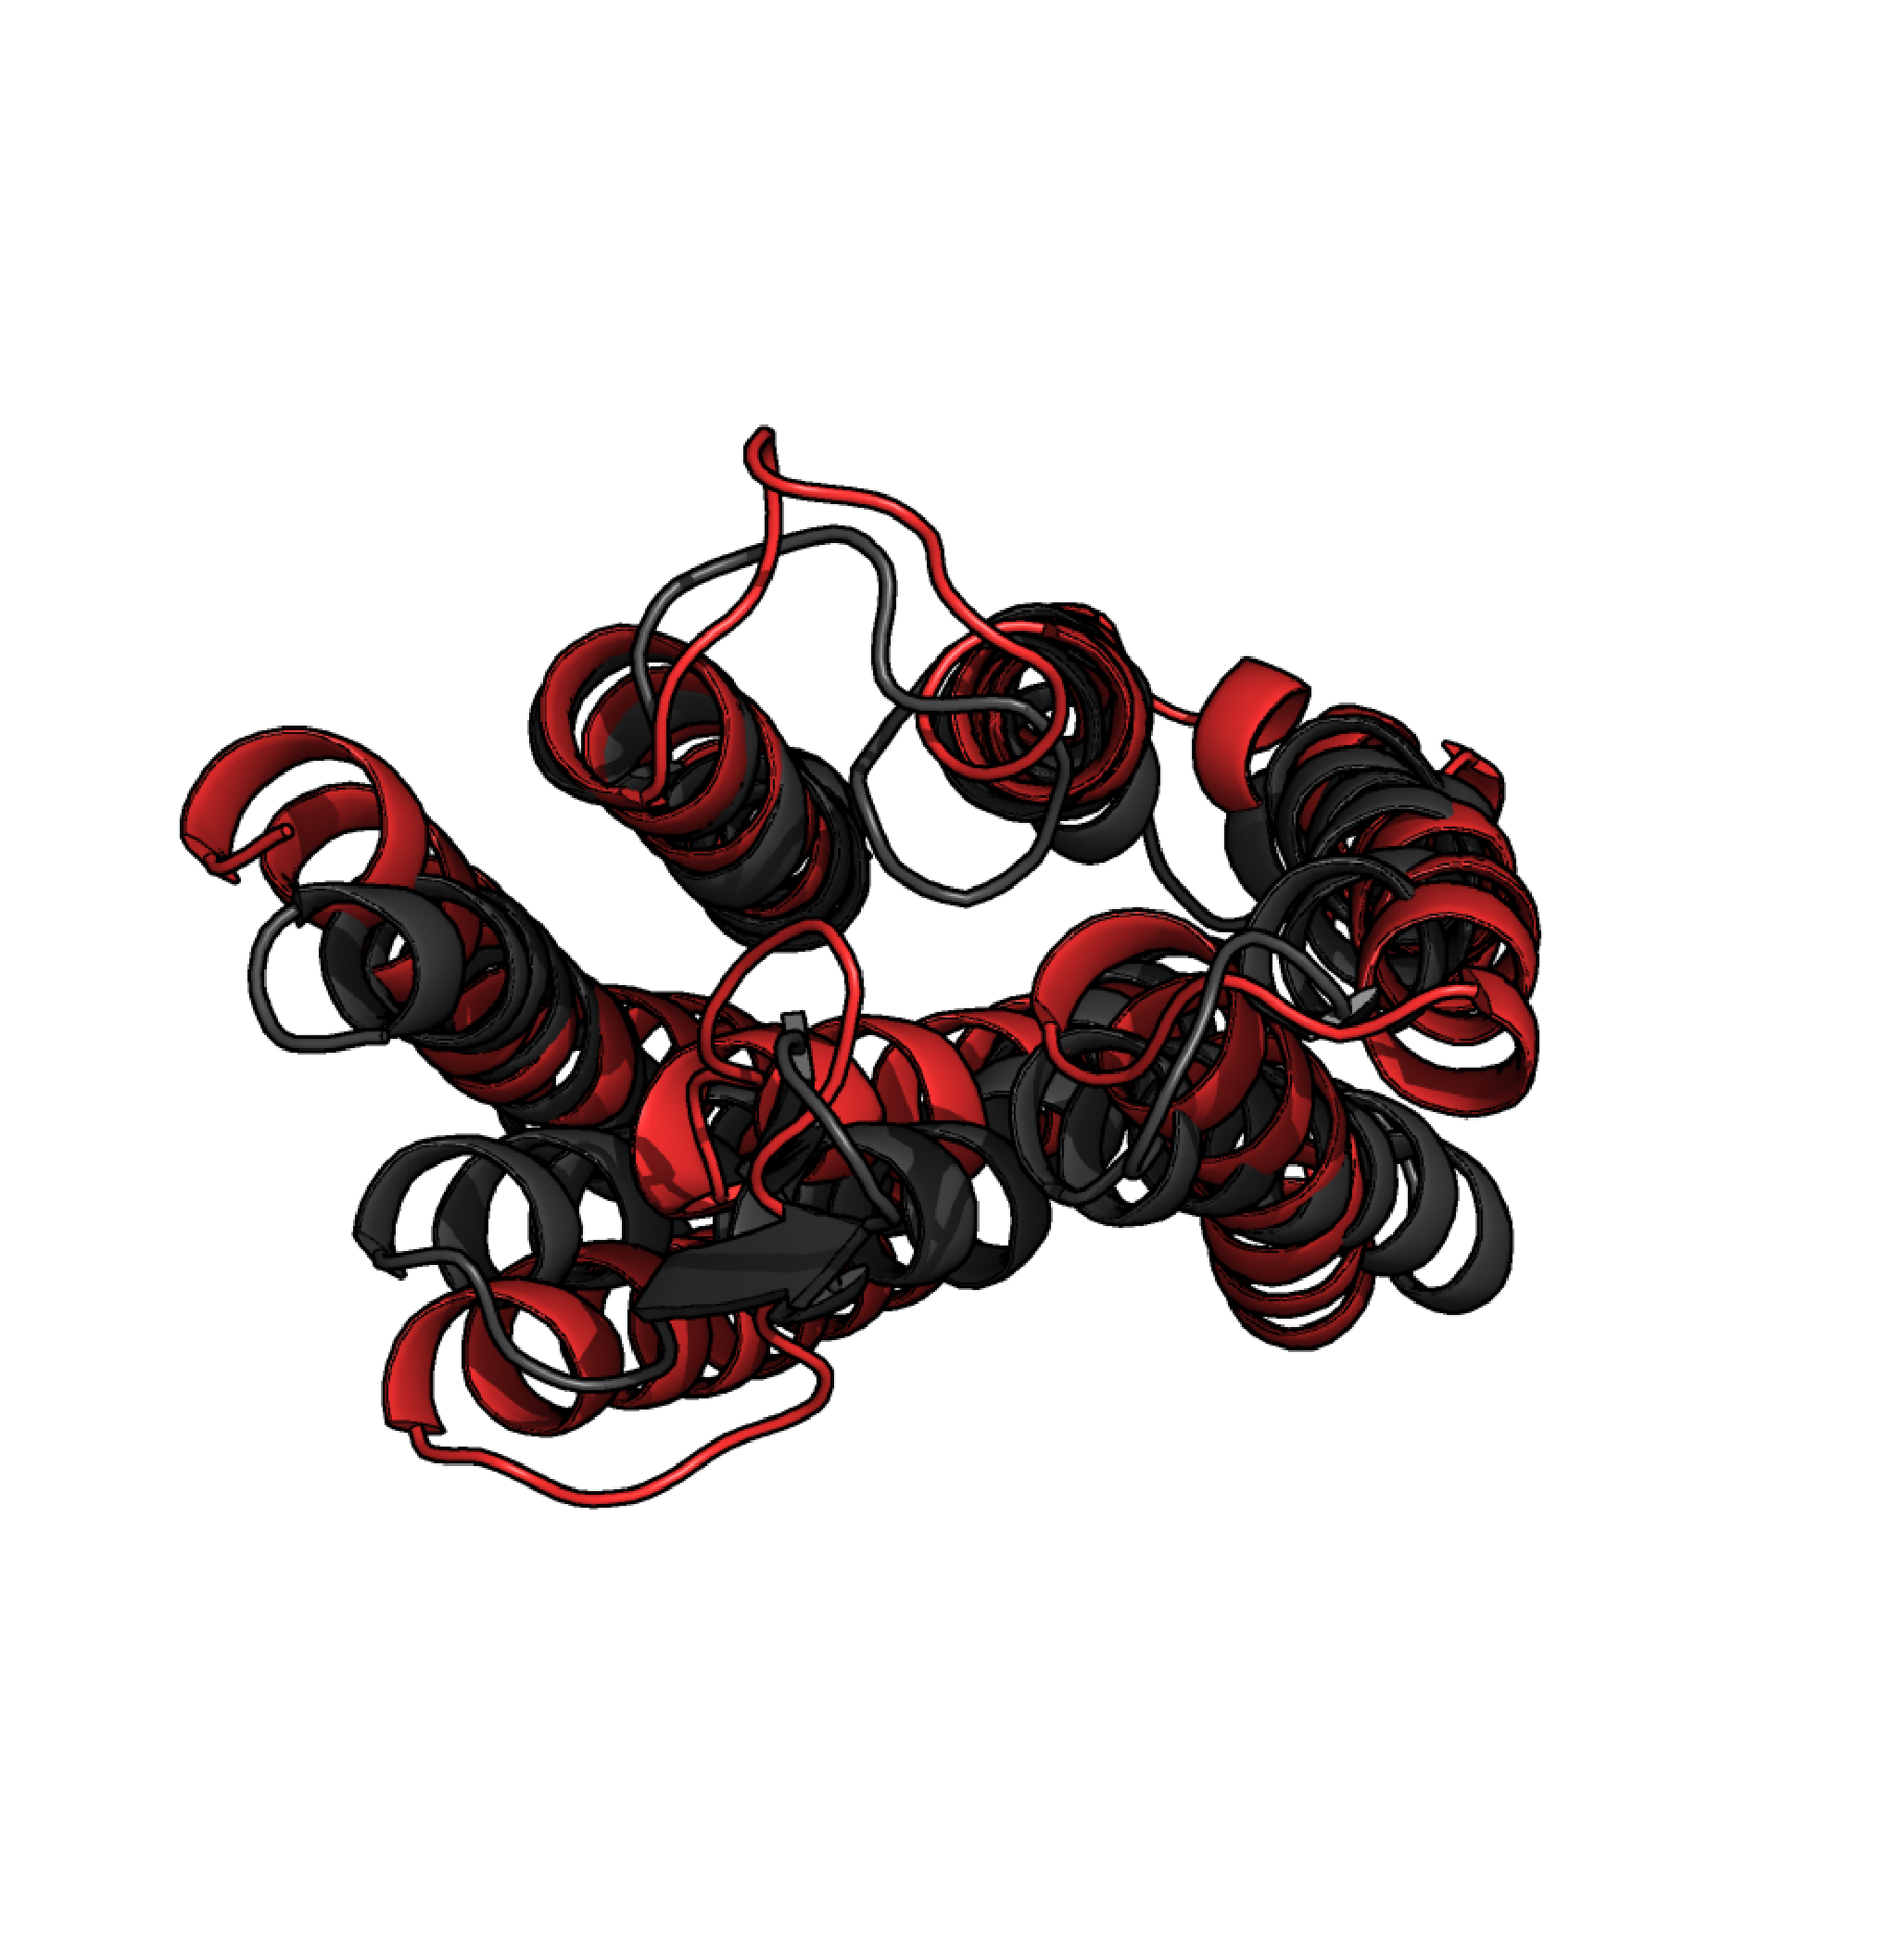
\includegraphics[width=0.4\textwidth]{figures/rhodopsin_figures/refinement_bottom.pdf}}
%    }\\
    \subfloat[Folding stage lowest energy sample (blue). 7.8 \AA~CA-RMSD.]{
        {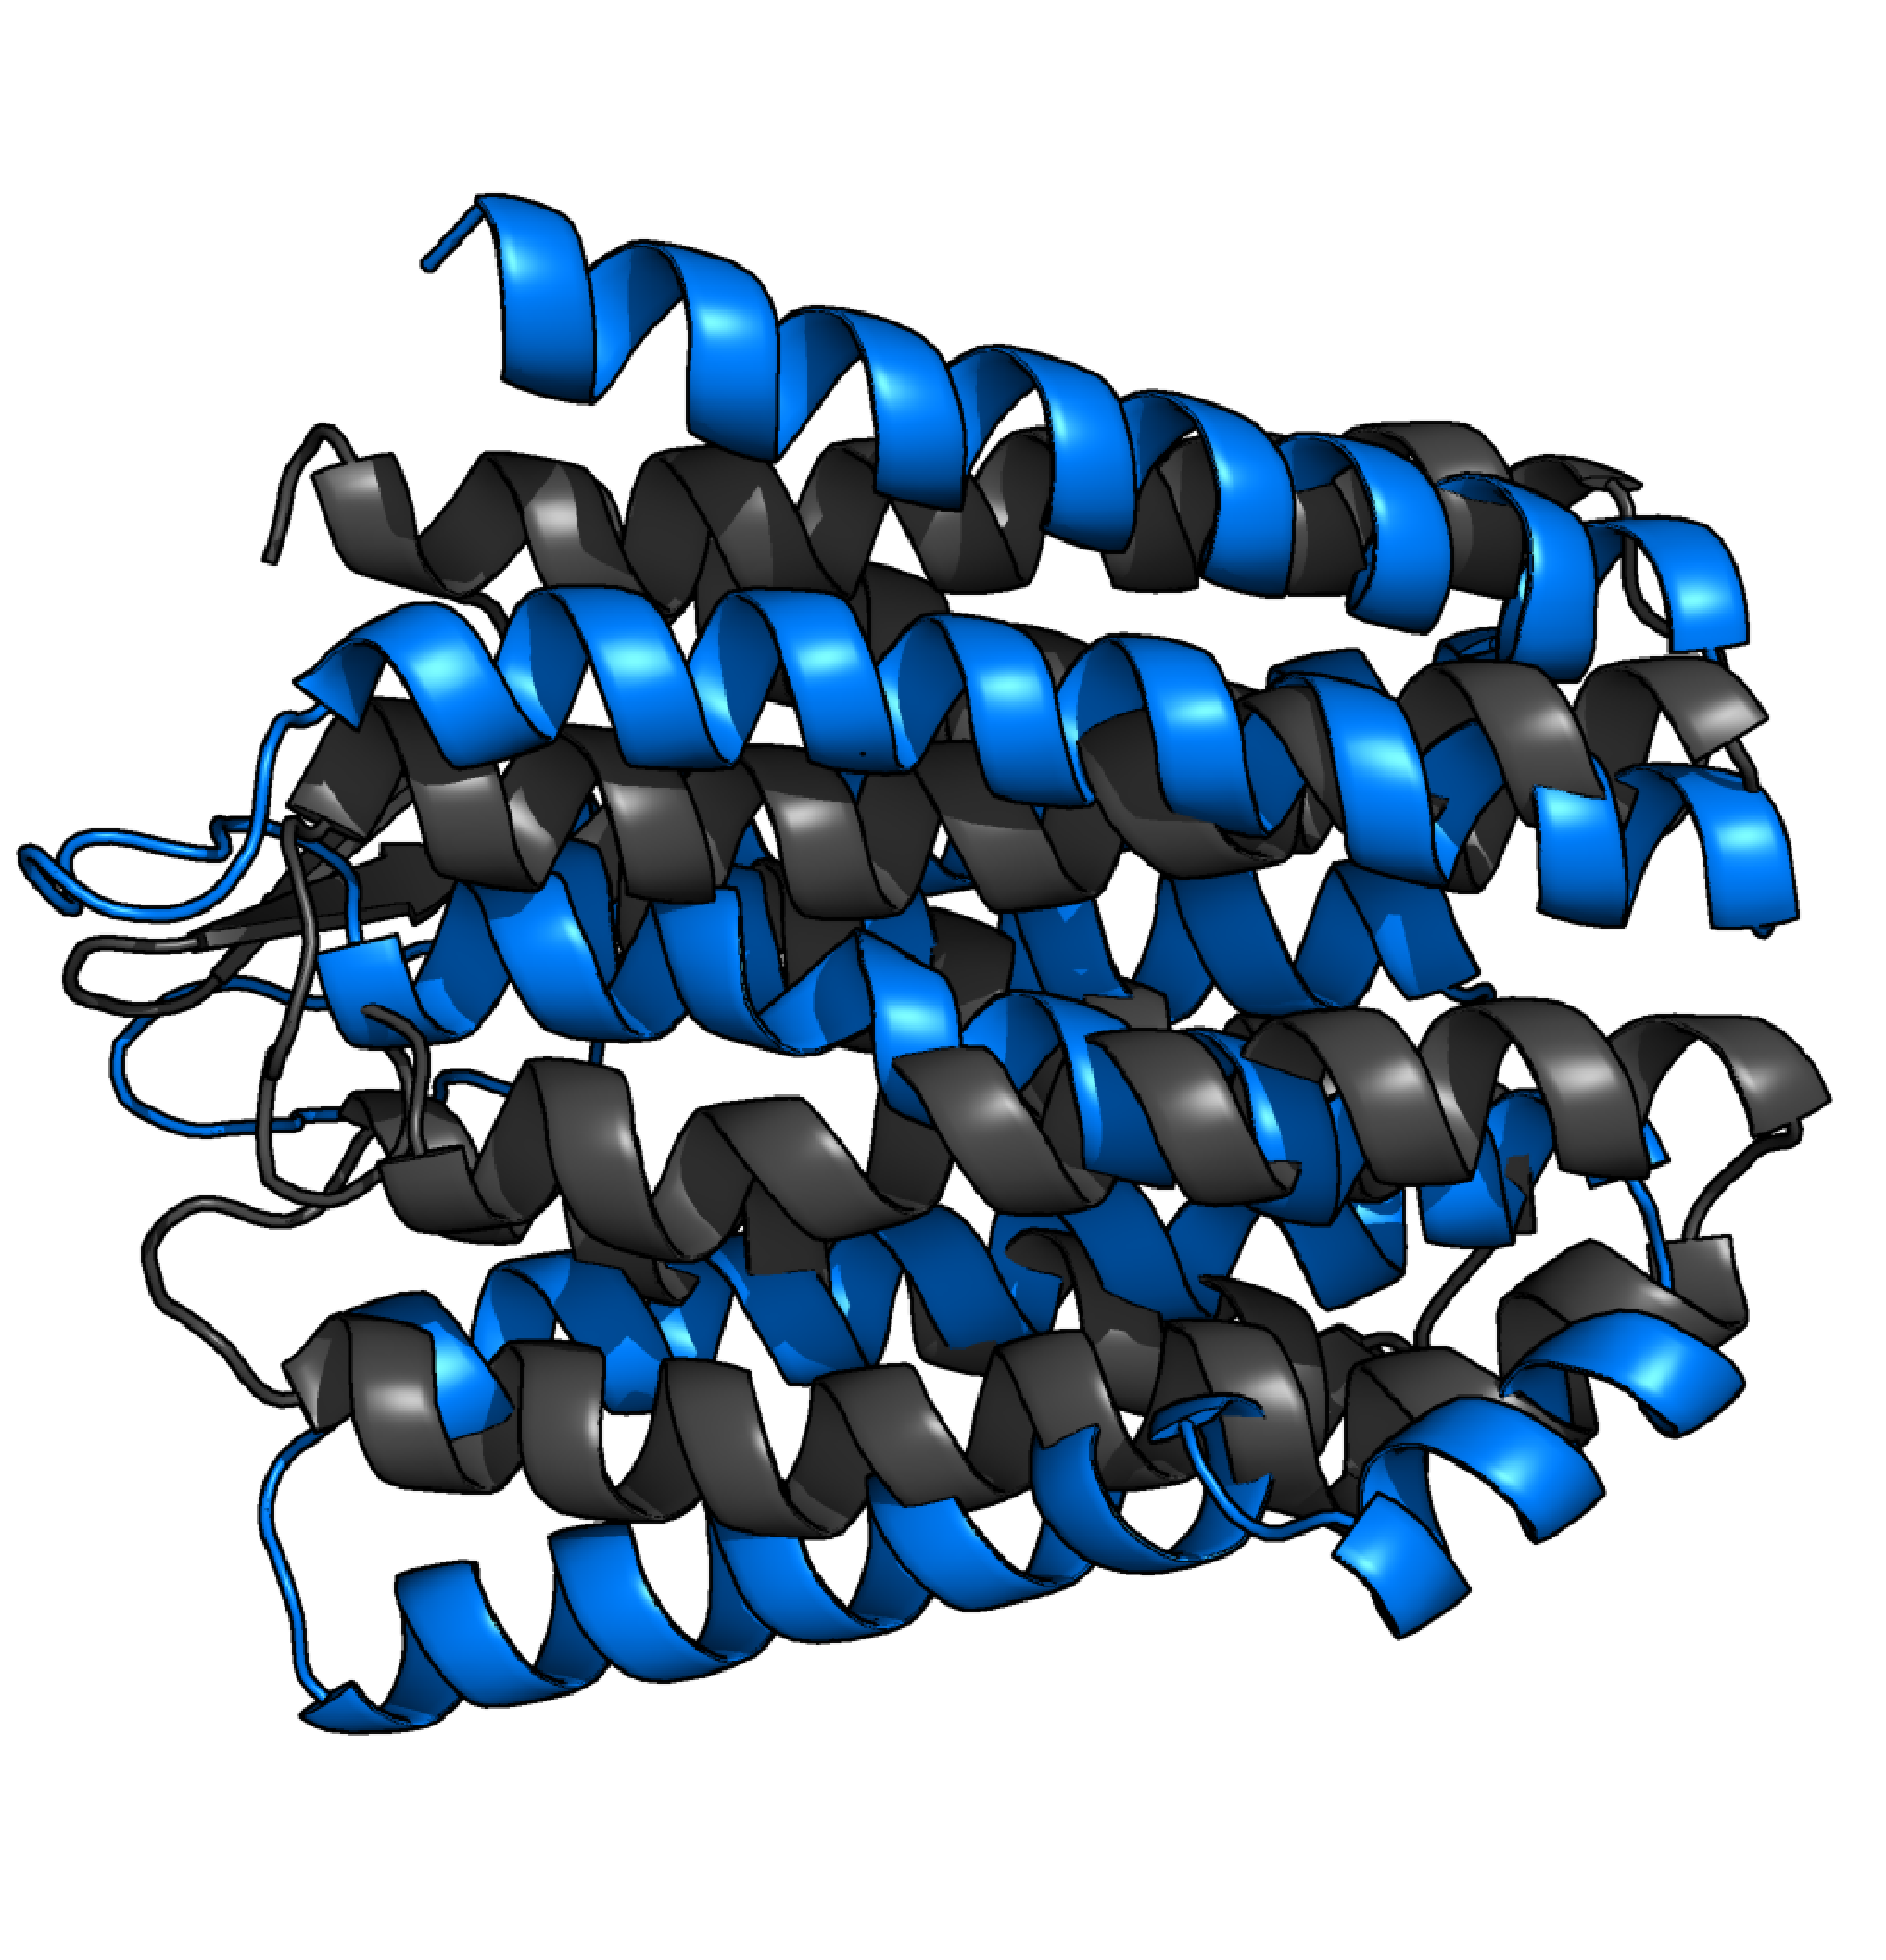
\includegraphics[width=0.4\textwidth]{figures/rhodopsin_figures/folding.pdf}}
    }\quad
    \subfloat[Refinement stage lowest energy sample (blue). 2.5 \AA~CA-RMSD. ]{
        {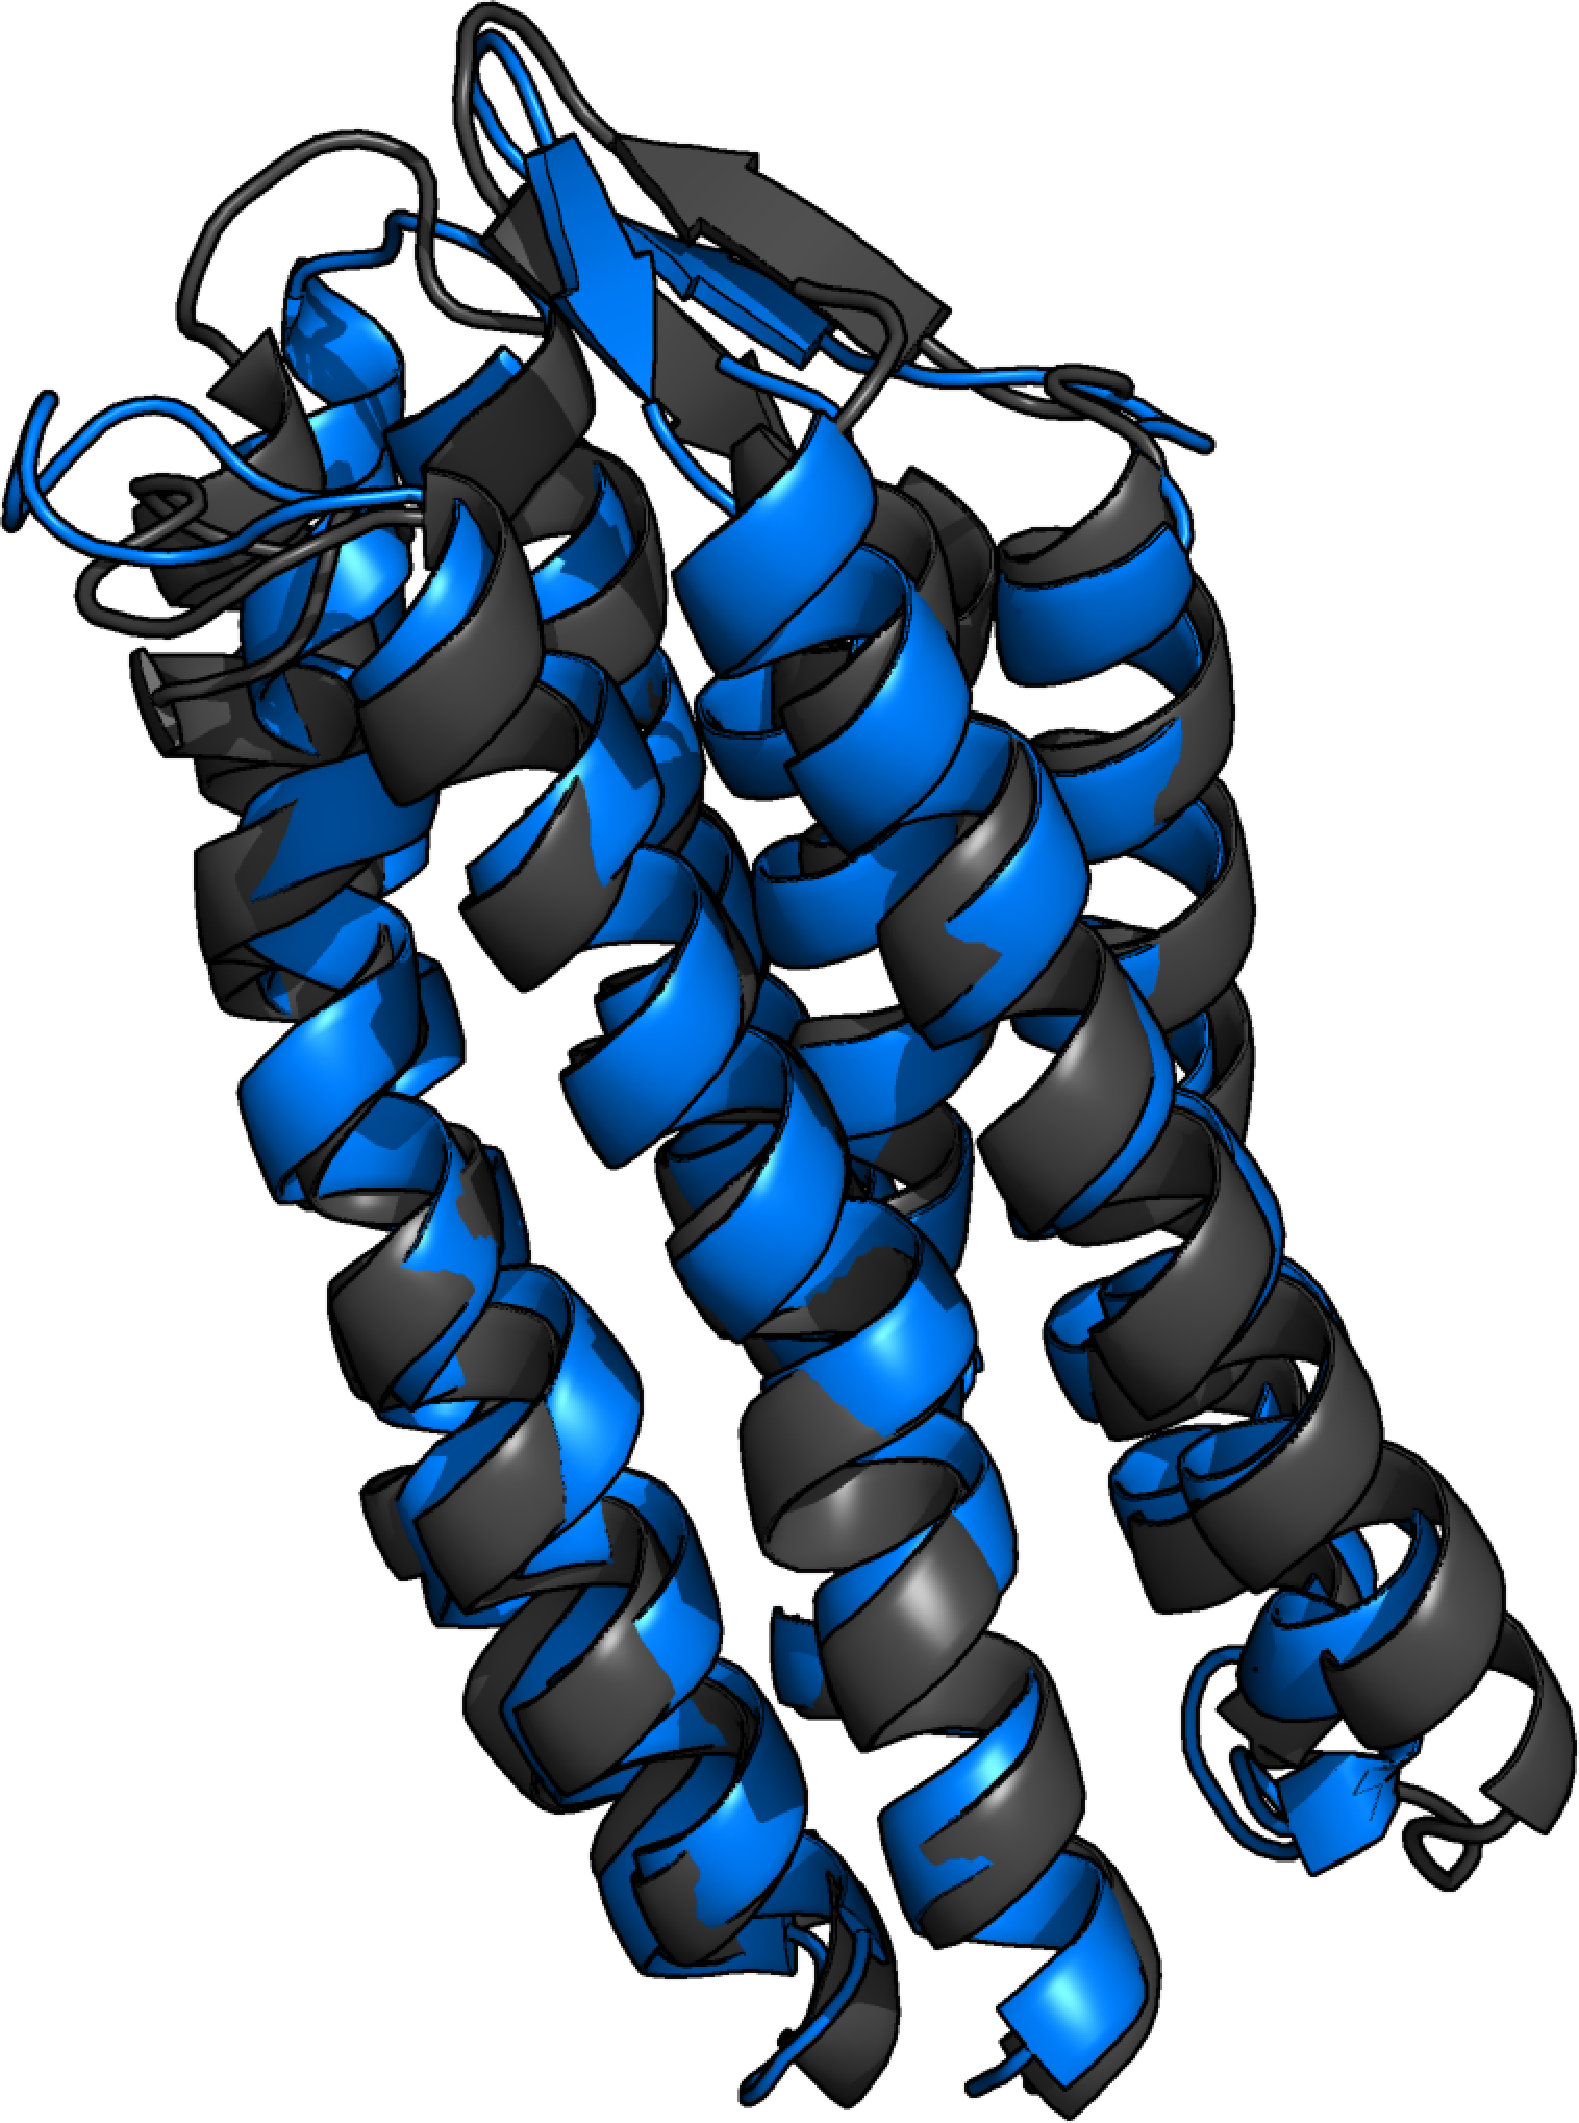
\includegraphics[width=0.4\textwidth]{figures/rhodopsin_figures/lowest_e.pdf}}
    }\\
    \caption{Some caption}
    \label{fig:rhodopsin}%
\end{figure}




\begin{table}[h]
    \caption{Folded structure.}
    \begin{center}
    \begin{threeparttable}
    \begin{tabular}{l l l l l l l}
Name                & Lengh    & Type   & PDB     & BMRB    & RMSD-range    &  RMSD  \\\hline
APO-LFABP           & 129      & a/b    & 1LFO    & 15429\tnote{a}  & All        &   \\
Prolactin           & 199      & B      & 1RWS    & 5599      & 6-183            &   \\
Top7                & 120      & a/b    & 2MBL    & 19404     & 5-104            &   \\
MSRB                & 151      & a/b    & 3E0O    & 17008     & 36-105           &   \\
WR73                & 183      & a/b    & 2LOY    & 16833     & 1-36,66-181      &   \\
HR4660B             & 174      & a/b    & 2LMD    & 1870      & 16-162           &   \\
Rhodopsin           & 219      & B      & 2KSY    & 16678     & All              & 3.2
    \end{tabular}
    \begin{tablenotes}
    \item[a] Data was obtained from RefDB.
    \end{tablenotes}
    \end{threeparttable}
    \end{center}
    \label{tab:folding_large}
\end{table}

Since the ILV(W) data set used by Rosetta was not available, simulated ILV restraints from the PDB structure 1h68 was used instead.
A very conservative simulation of only 63 synthetic NOE restraints was used, which corresponds to around 4\% assigned long-range contacts. The initial folding stage converged to around 6.8 as the lowest energy cluster - see Fig.~\ref{fig:rhodopsin}). Two threads out of 72 converged to this native-like cluster.

The refinement stage with only 63 NOEs, however, did not converge to a lower CA-RMSD.
The Rosetta data set includes 213 contacts, and a similar, less conservative synthetic NOE data was simulated from the PDB structure 1h68, in order to see, if an increased number of NOE restraints could drive the RMSD down.
 This resulted in 195 NOE restraints, which corresponds to 13\% assigned NOEs.
Using this, larger, set of restraints during the refinements gave a substantial decrease in CA-RMSD for the lowest energy sample to 3.6 \AA.

It must be noted, however, that in both the folding and refinment stages, samples are obtained with less than 2650 kcal/mol (calculated as the Profasi force field energy plus the likelihood from Torus-DBN-CS given the experimental chemical shifts), while the native energy is 2730 kcal/mol.
This discrepancy is likely due the lack of accurate non-local information in the Profasi and Torus-DBN-CS models.

Further refinement was attempted with the CamShift energy-term instead of the Torus-DBN-CS model, but was found to be too slow to be practically feasible.





\section{Evolutionary distance constraints}

\begin{figure}
    \centering
    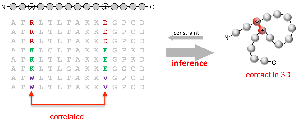
\includegraphics[width=0.85\textwidth]{figures/evo_constraint.pdf}
    \caption{Evolutionary constraints}
    \label{fig:evo_constraint}
\end{figure}

As discussed previously, it is increasingly difficult to obtain sufficient distance restraints as the size of the protein increases.
A recently developed methodology uses sequence analysis to infer residue contacts in 3D space. 

In brief, the method works by identifying sequence co-variation, which retains favorable contacts between residues.
This way, pair of residues which are probable to be close in 3D space can be identified.
The procedure is briefly summarized in Fig.~\ref{fig:evo_constraint}.

In this proof-of-concept study, 270 contacts were obtained a multiple-sequence alignment using the EVfold program (Wouter Boomsma, personal communications) for the 269 residue protein Savinase.
The restraints were simply treated as NOE restraints using existing code.
A similar simulation to that which folded Rhodopsin was adopted. 
In terms of computational resources, these were increased to 100 threads and $75 \times 10^6$ iterations, compared to only 72 threads and $50 \times 10^6$ iterations for the Rhodopsin simulation.
One thread identified a native-like structure.

The folding simulation yielded a lowest energy 


% \begin{figure}
%     \centering
%     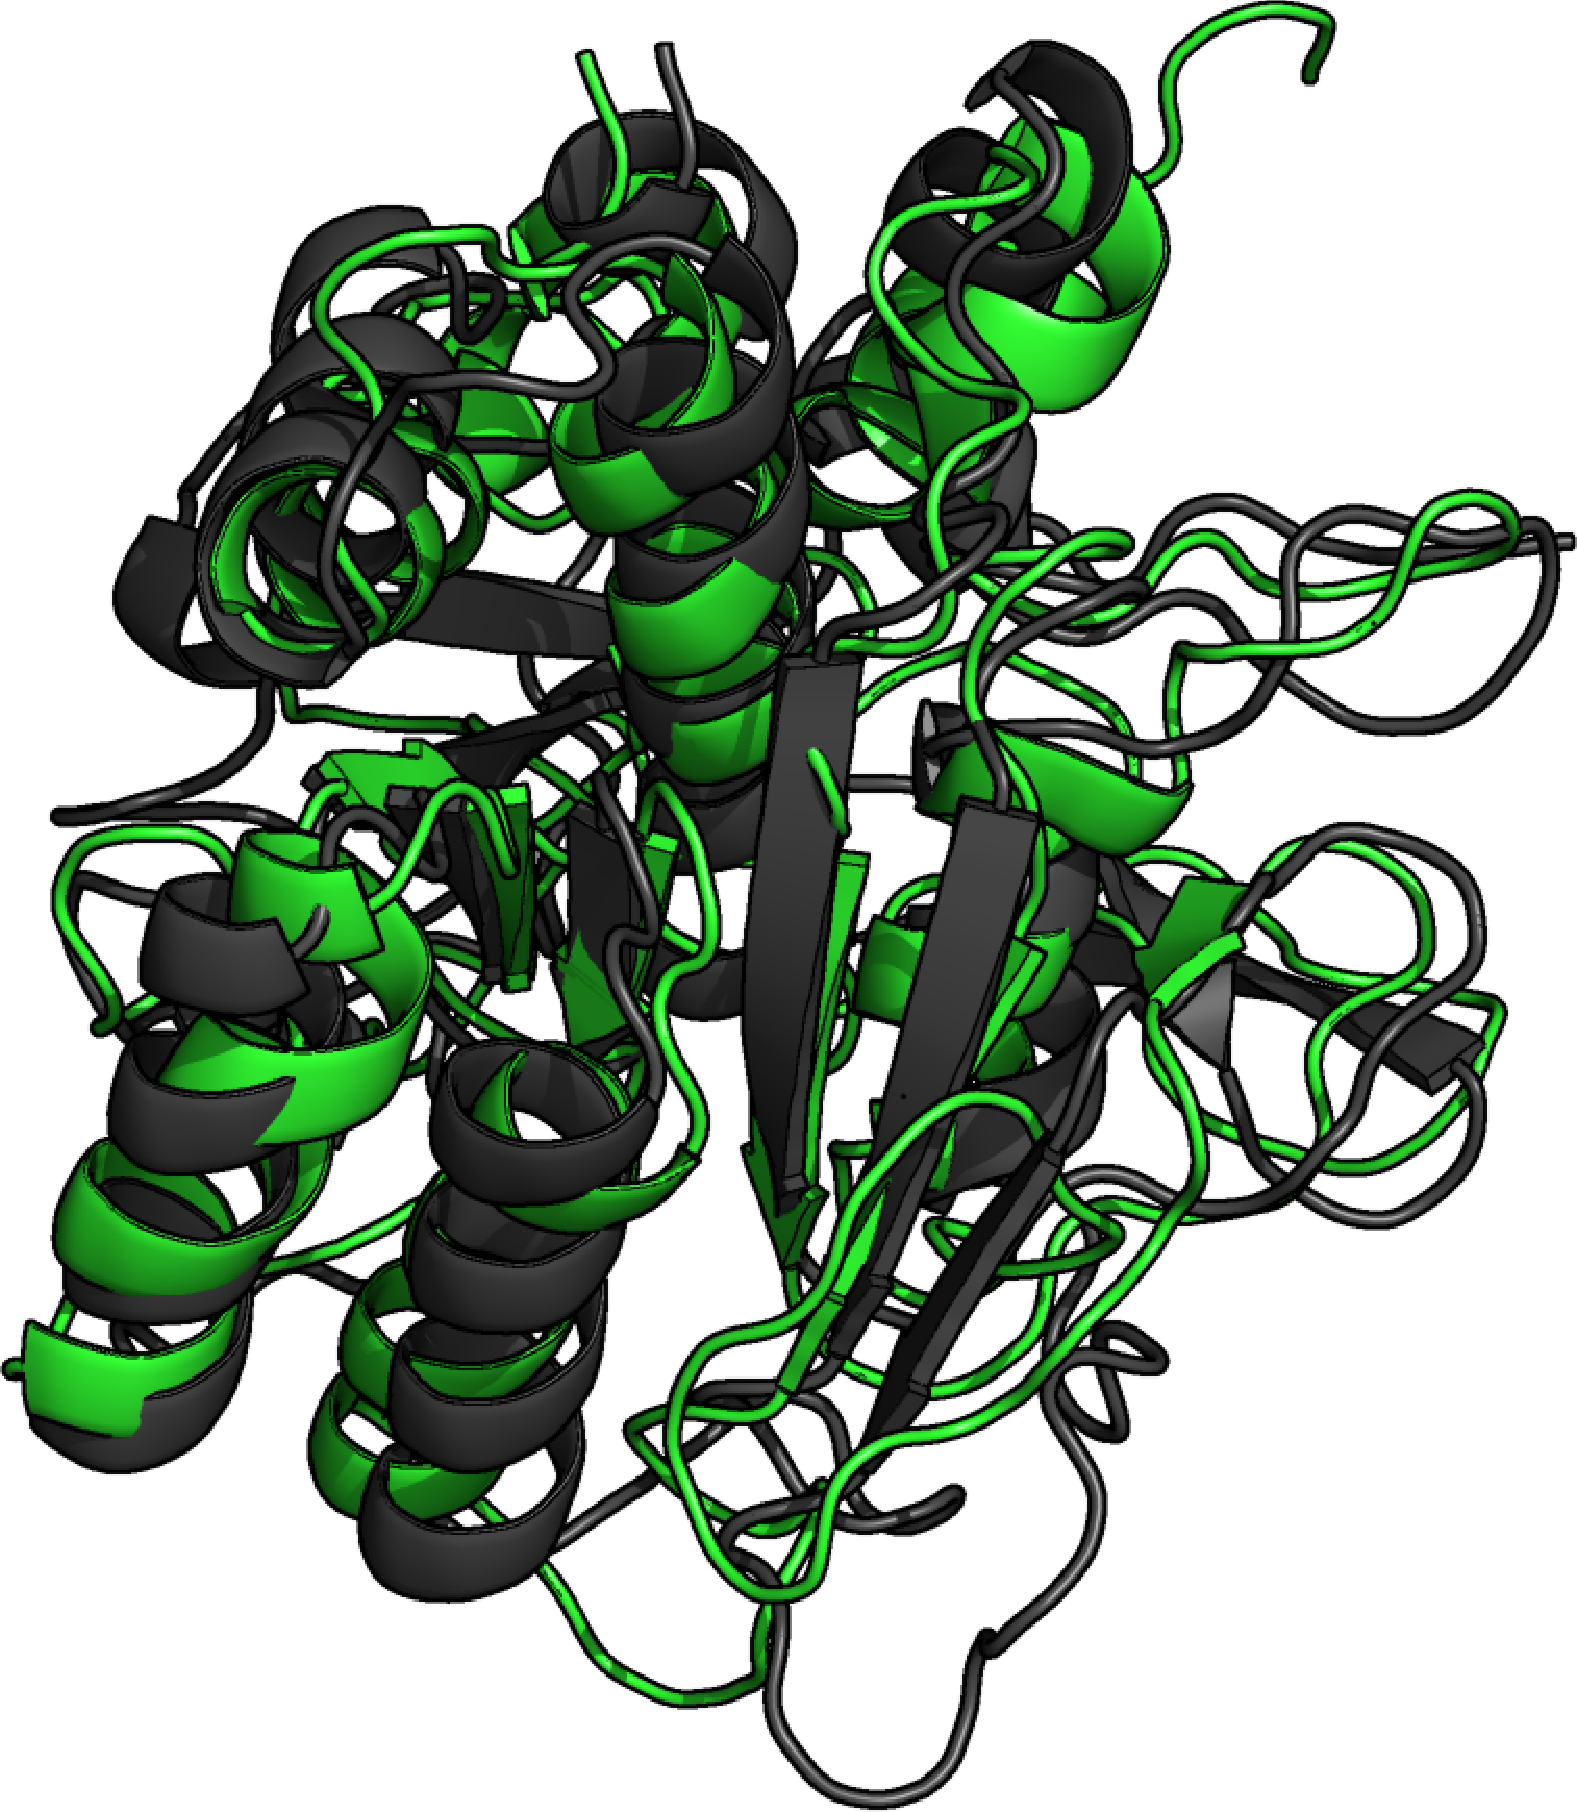
\includegraphics[width=0.60\textwidth]{figures/savinase_fold/savinase_lowest_e.pdf}
%     \caption{The lowest energy structure of Savinase after the refinement (green) and the 
%              1SVN crystal structure (grey). The CA-RMSD is 2.9 \AA.}
%     \label{fig:savinase_align}
% \end{figure}



\begin{figure}%
    \centering
    \subfloat[Lowest RMSD sample]{
        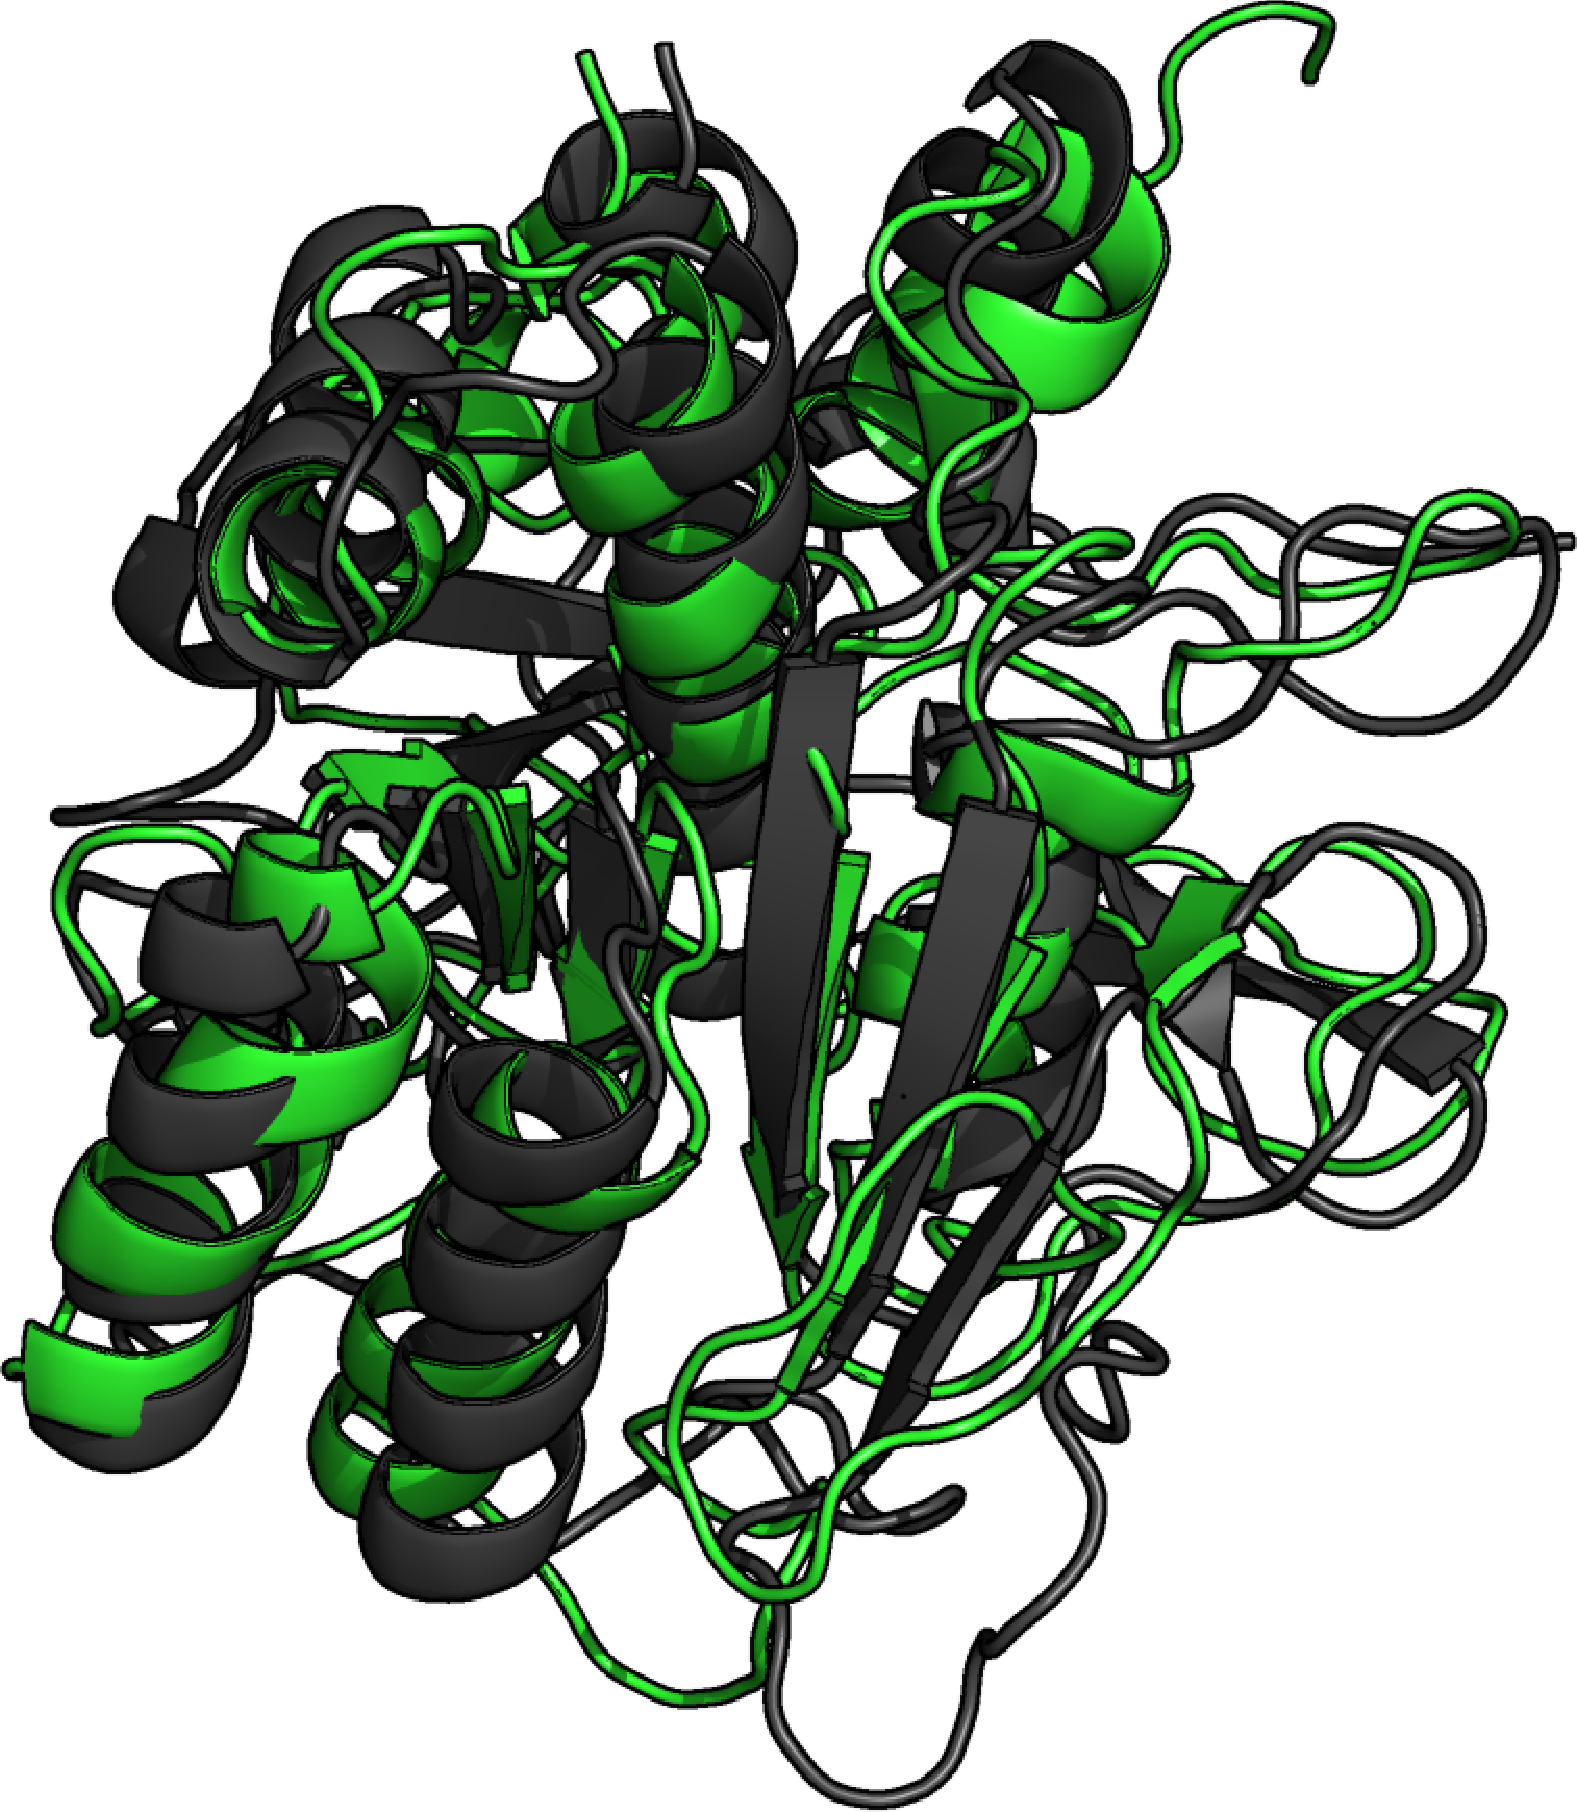
\includegraphics[width=0.40\textwidth]{figures/savinase_fold/savinase_lowest_e.pdf}
        %{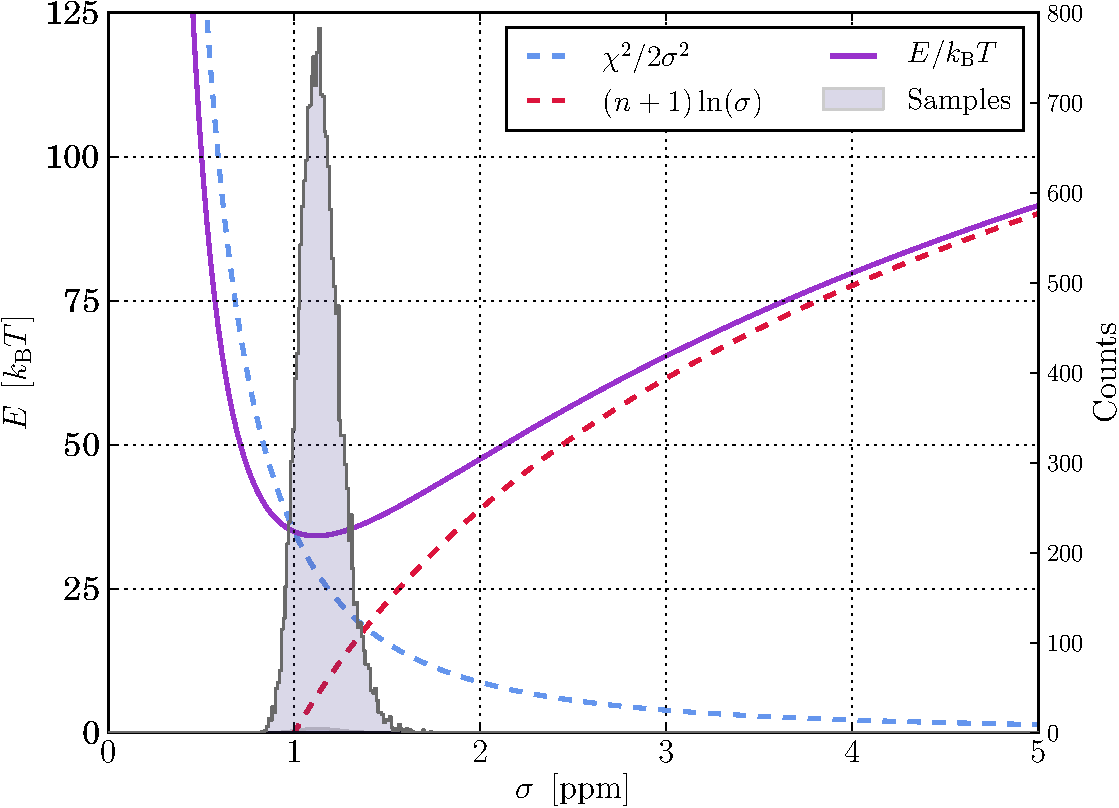
\includegraphics[width=0.42\textwidth]{sigma_prior.pdf} }
    }
    \subfloat[Lowest energy sample]{
        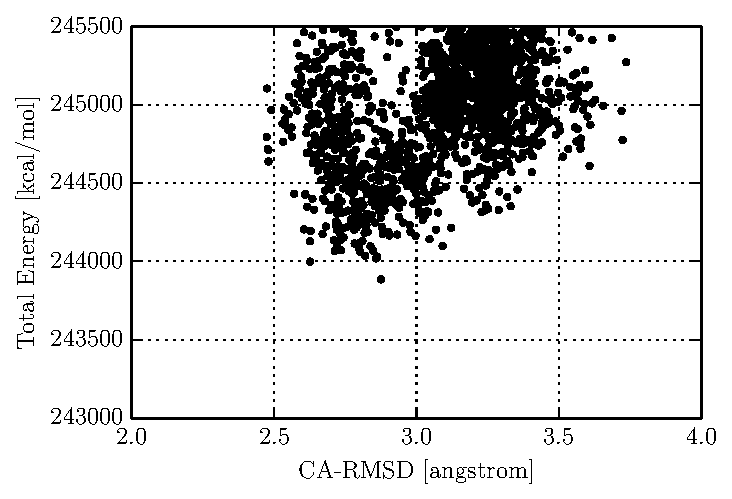
\includegraphics[width=0.60\textwidth]{figures/savinase_fold/savinase_refinement.pdf}
    }
    \caption{Refinement stage of the savinase simulation. The lowest energy sample has a CA-RMSD of 2.9 \AA. }
    \label{fig:savinase_fold}%
\end{figure}


% 
% \begin{figure}
%     \centering
%     \caption{Savinase folded}
%     \label{fig:savinase_align}
% \end{figure}
% 

